\subsection{A full-continuum thermal receiver for the actual O16 histories}
\label{sec:thermal-receiver-12}

The quantum-history claim now has a reconstructed continuum recipient.
Four original $K_4$ cores at $C_4$ address32 retain all 48 Gray signs and
eight currents. At times $j/8$, $j=0,\ldots,96$, HELD keeps the signs;
FORWARD flips $0,\ldots,47$ twice and REVERSE flips $47,\ldots,0$ twice.
All histories begin and end at $u=(4,0)^4$. Their equal-radius metrics are
\begin{equation}
\begin{gathered}
 G_{\rm edge}=(2I_4+J_4)\otimes I_2,\qquad
 G_{\rm outer}=J_4\otimes I_2/10,\\
 \tau_r=I_*=1.
\end{gathered}
\end{equation}
The source-to-wave calculation retains the complete shell continuum and
all 97 endpoint-inclusive events. For these classical alternatives only
the scalar nuclear-history phase is set to zero. A coherently controlled
superposition additionally requires its actual nuclear/Weyl phases.
\samref{REF12_FOUR}

Let $d=f_F-f_R$ be the difference of the two normal outgoing one-photon
amplitudes. Complete number and energy Grams give
\begin{align}
 \|d\|^2&\in[1266.24722856428927038757097294,\notag\\
 &\hspace{2.3em}1266.24722856428927038757097296],\\
 \langle d,\omega d\rangle&=3535/4.
\end{align}
The latter equality also follows from exact rational summation of the
triangle energy kernel over every difference event. Field works are
$26111/40$ and $25727/40$, with full ledger residuals containing zero.
All 48 contact means agree at observation16, although $d\ne0$.
Equal local means have therefore not removed the history record.

For $h=d/\|d\|$ and a supplied matched phase reference,
$X_h=(a(h)+a^\dagger(h))/2$ has coherent variance $1/4$ and mean
separation $\|d\|$. Midpoint discrimination obeys
$P_e=\Phi(-\|d\|)\le e^{-\|d\|^2/2}/2$.
Calibrated transmission $\eta$ replaces squared separation by
$\eta\|d\|^2$; collection and detector noise remain supplied inputs.

The original event differences satisfy exact moment cancellations
$M_0=\sum_j\Delta u_j=0$ and $M_1=\sum_jt_j\Delta u_j=0$.
Taylor's integral remainder gives
\begin{equation}
 \left\|\sum_j\Delta u_je^{i\omega t_j}\right\|_G
 \le\frac{\omega^2}{2}\sum_jt_j^2\|\Delta u_j\|_G.
\end{equation}
Cauchy over all events bounds the square of the last sum by
$10864751071/40$. With the same shell density and amplitude denominator
$\sqrt{2I_*\omega}$, its low-frequency number norm is
\begin{equation}
 N_{[0,.01]}\le M^2(.01)^4/(16\pi)<.054037.
\end{equation}
This bounds a squared norm. High-frequency positivity gives
$N_{(1,\infty)}\le883.75$, hence the sharpened complete band bound
\begin{equation}
 N_{[.01,1]}>382.443.
\end{equation}
It strengthens the earlier conservative $382.19596$ without introducing
a finite-frequency replacement for the continuum source.

Suppose the post-collection covariance is bounded as an operator by
$C(\omega)=\coth(\beta\omega/2)$ and signal power transmission is
calibrated as $\eta$. The matched Gaussian filter is proportional to
$C^{-1}d$, with squared effective separation
\begin{equation}
 Q=\eta\langle d,C^{-1}d\rangle
 \ge\eta\tanh(.01\beta/2)N_{[.01,1]}.
\end{equation}
At $\beta=200$, $\eta=1/40$, the native compiled recipe gives
$Q>7.28165884465476$ and $P_e<.013115290<.01312$.
The earlier band separately gives $P_e<.01315$. Mean efficiency or mean
noise does not establish the required positive-operator inequalities.
Physical temperature/frequency scales, collection, mode shaping, phase
locking, apparatus energy and reset are not assigned by this certificate.

\begin{figure}[htbp]\centering
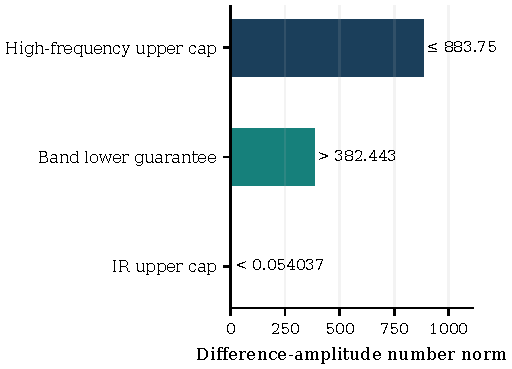
\includegraphics[width=\columnwidth]{refinement_20261112/figures/continuum_receiver.pdf}
\caption{A guaranteed band of the full F/R difference record. Total
number norm is enclosed; low- and high-frequency values are upper caps,
leaving a lower guarantee in $[.01,1]$. The companion receiver bound
requires the stated covariance, phase reference and transmission.}
\label{fig:continuum-receiver-12}
\end{figure}

\subsection{Two amplitude modes retain this dictionary's distinctions}
\label{sec:dictionary-12}

For any fixed coherent dictionary $f_1,\ldots,f_M$, remove a common
displacement and span $d_j=f_j-f_1$. Their normal Gram has rank
$r\le M-1$. An orthonormal basis of this span extends to a passive
one-photon unitary; the orthogonal coherent factor is common to every
hypothesis and can be discarded without losing their statistical
distinction. For the actual HELD/FORWARD/REVERSE dictionary, the difference
Gram is rank two with determinant greater than
$1837116.41394784$. Binary F/R requires one matched direction.
These are complete amplitude modes with infinite Fock spaces, not two
frequencies or a finite-dimensional quantum state. The phases mentioned
above must accompany a controlled quantum superposition. The finite
dictionary rank is a statistical receiving statement with its physical
mode-control implementation still specified separately.
